\documentclass[../../main.tex]{subfiles}

\begin{document}

\section{Motivation}

Machine learning models have been immensely successful in variety of applications to generate predictions in data-driven driven domains such as computer vision, robotics, weather forecasting. While the success of these models is undeniable, we lack the ability to understand the uncertainty in the predictions made by most of the State-of-the-Art models. This is a major drawback in the deployment of these models in real-world applications, for example, in weather forecasting, it is important to know the uncertainty in the prediction of the weather as this information is arguably as valuable as the prediction itself. In this work, we aim to implement a model is \textbf{Uncertainty Aware} whilst also possessing further desirable properties.

\section{Desirable Properties}

Onto of being uncertainty aware, we would like to insert some desirable inductive biases that help the model to generalize better and be more interpretable. We would like the model to be able to:

\textbf{Flexible}: \emph{The model should be able to work on a variety of data types}. As long as a data point can be represented as a vector, the model should be able to work on it. This allows the model to be used in a variety of applications and domains.

\textbf{Scalable}: \emph{The model should be able to work on large datasets}. The model can be trained on large datasets and should be able to make predictions on large datasets. There should be no limit on the size of the dataset that the model can work on which is not the case with many traditional models such as LLMs. Another aspect of scalability is the ability to work on high-dimensional data and large data sets with good computational efficiency.


\textbf{Permutation Invariant}: \emph{The prediction of the model should not change if the order of the input data is changed}. When each data point contains the information about input and output pairs, the model should not care about the order in which they are fed into the model. For example, in the case of a weather forecasting model using data from multiple weather stations, the model should not care about the order in which the data from the weather stations is fed into the model, thus making the model permutation invariant.

\textbf{Translation Equivariant}: \emph{Shifting the input data by a constant amount should result in a constant shift in the predictions}. For example, in the case of a weather forecasting model, if the data from the weather stations is shifted by a constant amount, the model should be able to predict the same shift in the weather forecast.

\begin{figure}[H]
	\centering
	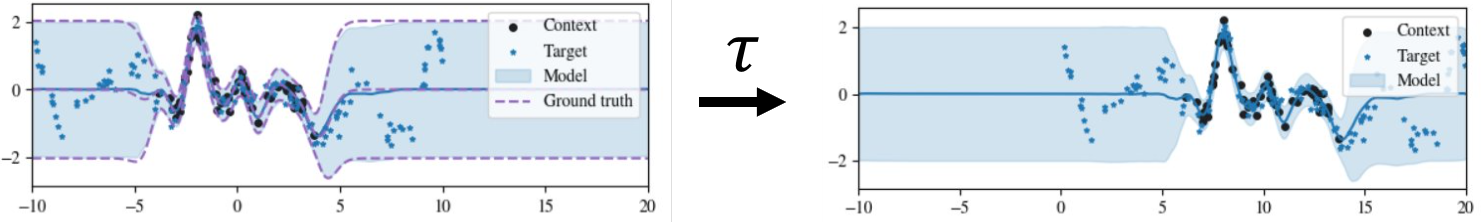
\includegraphics[width=0.9\textwidth]{./te.PNG}
	\caption{The Translation Equivariant property. Consider the given prediction on the black data points on the left. If the input is shifted by a constant amount, the prediction should also shift by the same amount (right).}
	\label{fig:te}
\end{figure}


\todo{Clearer figure}

\autoref{fig:te} illustrates the Translation Equivariant (TE) property on a simple 1D dataset. If the model, $f$ is TE then the following holds:

\begin{align}
	&f: \bm{x} \rightarrow (\bm{x}, \bm{\hat{y}}) \\
	&f: \bm{x} + \bm{c} \rightarrow (\bm{x} + \bm{c}, \bm{\hat{y}})
\end{align}

Where $\bm{x}$ is the input and $\bm{\hat{y}}$ is the output and $\bm{c}$ is a constant shift in the input.


\textbf{Off-the-Grid Generalization}: \emph{The model should be able to work on off-the-grid data points}. Off-the-grid data points are the data points that are not in a regular gridded structure, for example, images that are missing pixel values are off-the-grid. Traditional models like Convolutional Neural Networks (CNNs) are not able to work on off-the-grid data points since they require a regular structure to apply the convolution operation. By making the model off-the-grid generalizable, we can create models that can work on many types of data and easily handle missing data points. It also allows the model to generalize to regions of the input space that it has not seen during training. Tasks like image inpainting, where the model is required to fill in missing pixels in an image, can benefit from this property.

\todo{Add a figure to illustrate off-the-grid generalization}

\section{Aims and Objectives}

Neural Processes (NPs) \cite{garnelo2018neural} are a class of models that satisfy the above properties. The framework undermining NPs is general purpose and thus it can be modified with a variety of neural network architectures. 

In this work, we aim to implement and compare two different neural network architectures for Neural Processes, the first being based on a Convolutional Neural Network (CNN) called Convolutional Neural Processes (ConvNP) and the second being based on a Transformer architecture called Transformer Neural Processes (TNP). We aim to compare the two models on a variety of tasks and datasets to see how they perform in terms of generalization, scalability, and uncertainty estimation. 

Furthermore, we investigate how the TNP can be optimized to achieve better performance. We then investigate new Transformer architectures that have better computational efficiency compared to the original Transformer architecture. 

Our end goal is to better understand the properties of these models and how they can be used in real-world applications and figure out the best practices for using these models in different scenarios. 





\ifSubfilesClassLoaded{%
    \printbibliography{}
}{} 


\end{document}